\documentclass[12pt,a4paper]{article}
\usepackage{lmodern}
\usepackage[utf8]{inputenc}
\usepackage[T1]{fontenc}
\usepackage{geometry}
\usepackage{setspace}
\usepackage{graphicx}
\usepackage{hyperref}
\geometry{a4paper, total={170mm,257mm}, left=20mm, top=20mm}

\title{\Huge BaDMat 1.0 \\ \LARGE Mode d'emploi} % Ça fait un peu BatMan, on garde vraiment ce nom-là ?
\author{Myrtille Grulois \thanks{Université populaire et citoyenne de Roubaix}}
\date{Été 2020}

\renewcommand*\contentsname{Sommaire}

\begin{document}

\begin{titlepage}
    \maketitle
\end{titlepage}

\tableofcontents
\clearpage

\addcontentsline{toc}{section}{Introduction}
\section*{Introduction}

    Ce manuel d'utilisation concerne la première version du logiciel BaDMat de l'UPC de Roubaix.
    Les explications concernent à la fois la structure de la base de données et les différentes fonctions disponibles.
    Pour toute action d'ordre général, se reporter au préambule, qui contient des instructions valables pour la plupart des fonctions (sauf mention contraire).

\bigskip
\section{Préambule : ce qu'il est utile de savoir (faire)}
    
    \subsection{Ouverture de l'invite de commande}
    
        Bon je vais pas trop détailler, comme on n'a pas encore décidé de l'OS à utiliser\dots
        %TODO À mettre à jour.
    
    
    \bigskip
    \subsection{Lancement d'un script}
        Tout d'abord, précisons que dans notre cas, un script correspond à une fonctionnalité.
        Chaque fonction décrite ci-dessous est donc lancée à partir d'un fichier différent.
        Pour lancer un script (à compléter, dépend 1. de l'OS 2. de comment fonctionne Python sur l'OS)
        %TODO
    
    \bigskip
    \subsection{Utilisateurs et connexion à la base de données via Python}
        Pour consulter la base de données, il vous suffit d'entrer \emph{user} lorsqu'on vous demande l'utilisateur.
        Pour toute autre action, vous aurez besoin d'un compte avec des droits étendus.
        Pour cela, reportez-vous à la personne chargée de créer les comptes, ou bien à la section correspondante de ce manuel.
        Une fois que vous disposez d'un nom d'utilisateur et d'un mot de passe, vous pouvez effectuer le script de
        votre choix en entrant vos identifiants lorsqu'ils sont demandés. Pour la recherche, continuez à utiliser l'utilisateur commun \emph{user}.
    
    
    \bigskip
    \subsection{Interactions avec le programme}
        Pour la plupart des instructions, le programme nécessite que vous rentriez une lettre en majuscule.
        Tapez la lettre correspondant à votre choix parmi les propositions de la question,
        puis validez en tapant \emph{Entrée}.
        Parfois, on vous demandera également de taper \emph{Entrée} pour toutes les colonnes que vous
        souhaitez passer, et n'importe quelle lettre pour toute autre action.
        De manière générale, une instruction précède à chaque fois les commandes à entrer
        pour vous guider.
    
    
    \bigskip    
    \subsection{Définition des termes utilisés}
        On parlera plus loin de table lorsqu'on parlera de catégorie enregistrée dans la base de données :
        ainsi, il y aura par exemple une table pour les différents matériaux, et une autre pour les pièces
        qui sont composées de ces matériaux.
    
        Tout au long de la suite, ligne désignera une entrée dans la base de données.
        Colonne désignera un des possibles critères de cette ligne (le nom, la taille, la quantité\dots)
        
        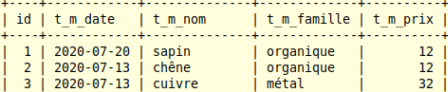
\includegraphics{exemple_lignes_colonnes.png}
    
        Dans l'exemple ci-dessus, vous avez un extrait de la table des matériaux.
        Une ligne de cette table (par exemple celle d'ID 1 décrivant le sapin) correspond à une entrée
        dans la table, donc à un matériau. Elle sera nommée\dots ligne.
        On nommera colonne, par exemple, le critère ID. Pour aller plus loin, la colonne ID
        est de type numérique, tandis que la colonne t\_m\_famille est de type textuel.
        Reportez-vous à la section \textbf{Base de données} pour connaître plus précisément
        les types de chaque colonne, ainsi qu'aux \textbf{Annexes} pour une description
        de chaque type.
    
    
    
\clearpage
\section{Fonctions}

    Cette section regroupe les différentes fonctions implémentées, ainsi que la façon de les exécuter, et les différentes options possibles.

    \bigskip
    \subsection{Recherche}\label{recherche}

        La fonction principale de cette base de données est la fonction de recherche.
        Pour l'exécuter, lancer le script \emph{search.py}, puis se connecter à la base de données.
        Pour vous connecter, utilisez \emph{user} comme identifiant, pour lequel on ne vous demandera
        pas de mot de passe.
        Vous devrez commencer par choisir dans quelle table est-ce que la recherche s'effectuera.
        Il existe deux types de recherche : la recherche simple et la recheche avancée.

        \subsubsection{Recherche simple}
            La recherche simple est à privilégier si vous ne souhaitez inclure qu'une seule colonne dans votre recherche.
            Vous aurez toujours la possibilité de choisir quelle(s) colonne(s) vous souhaitez afficher dans les résultats.


            \medskip
            \textbf{Recherche textuelle}

            Si la colonne que vous sélectionnez est de type textuel, alors vous pourrez entrer un mot ou une expression.

            \medskip
            \textbf{Recherche numérique}

            Si la colonne que vous sélectionnez est de type numérique, vous pourrez effectuer une recherche autour d'une valeur donnée,
            ou bien une recherche sur un intervalle. Si vous choisissez la recherche numérique simple, vous aurez toutefois
            la possibilité d'entrer une tolérance. La recherche s'effectuera alors sur l'intervalle de longueur de deux fois votre tolérance
            qui entoure votre valeur.
            Si vous rentrez une valeur décimale, pensez bien à saisir un point (.) et non une virgule.

            \medskip
            \textbf{Recherche par date}

            Vous pouvez également effectuer une recherche sur la date.

        \subsubsection{Recherche avancée}
            La recherche avancée vous prendra plus de temps. Elle permet à la fois d'effectuer une recherche sur plusieurs colonnes,
            mais également de rechercher plusieurs critères dans la même colonne (pour les colonnes de texte).

            \medskip
            \textbf{Recherche textuelle}

            Si la colonne que vous sélectionnez est de type textuel, alors vous pourrez entrer un mot ou une expression, qui sera recherché
            dans cette colonne. Toutefois, vous aurez ensuite la possibilité d'ajouter des mots supplémentaires, que vous pourrez moduler :
            c'est-à-dire imposer que le mot saisi ne se trouve pas dans les résultats de votre recherche, ou bien cherche le premier terme
            ou bien le deuxième, etc.

            \medskip
            \textbf{Recherche numérique}

            La recherche numérique avancée est identique à celle de la recherche simplifiée.
            Si la colonne que vous sélectionnez est de type numérique, vous pourrez effectuer une recherche autour d'une valeur donnée,
            ou bien une recherche sur un intervalle. Si vous choisissez la recherche numérique simple, vous aurez toutefois
            la possibilité d'entrer une tolérance. La recherche s'effectuera alors sur l'intervalle de longueur de deux fois votre tolérance
            qui entoure votre valeur.

            \medskip
            \textbf{Recherche par date}

            Vous pouvez également effectuer une recherche sur la date.

        \bigskip
        Une fois que vous aurez entré vos critères de recherche, vous pourrez
        également choisir les colonnes à afficher, et ce quel que soit le type
        de recherche préalablement choisi. Pour cela, vous avez trois
        possibilités : afficher les colonnes par catégorie (description de ces
        dernières dans l'annexe \nameref{structureinitiale}, afficher toutes les colonnes (ce type
        d'affichage est déconseillé la plupart du temps), ou encore afficher des
        colonnes que vous sélectionnerez manuellement.


    \bigskip
    \subsection{Ajouter une nouvelle ligne}\label{ajoutligne}

        Lorsque vous souhaitez ajouter une nouvelle ligne, il vous faut utiliser le script \emph{addRow.py}.
        Connectez-vous, puis indiquez quelle table vous souhaitez compléter.
        On vous demandera ensuite d'entrer un par un les critères que vous souhaitez compléter.
        Si pour un critère donné vous ne savez pas, vous pouvez simplement taper "Entrée".
        Cela laissera vide la colonne concernée.
        Toutefois, certaines colonnes ne peuvent pas être laissées vides. Pour celles-là (plus de précisions dans
        l'annexe \nameref{structureinitiale}), il faut impérativement que vous entriez une valeur.

        La complétion de certaines colonnes est conditionnée par des termes préalablement rentrés. Par exemple,
        il ne vous est pas possible d'entrer une pièce composée d'un matériau qui n'est pas présent dans la base
        de données. Il faudra d'abord que vous créiez le matériau, puis vous pourrez ajouter la pièce associée.
        Le même principe s'applique pour la famille de matériaux. Un certain nombre de termes est autorisé (organique,
        métal, alliage, composite, polymère, céramique). Si vous essayez de rentrer un autre terme, vous obtiendrez une
        erreur. La liste complète des colonnes contraintes est consultable dans l'annexe \nameref{structureinitiale}.
        Pensez à tenir cette annexe à jour si vous souhaitez continuer à ce qu'elle soit pertinente.
        En outre, le script \emph{printTerms.py} vous permet d'afficher la liste actuelle des termes autorisés.

        Si vous entrez une valeur décimale dans les colonnes qui l'acceptent, pensez bien à utiliser le point et non la
        virgule comme séparateur.


    \bigskip
    \subsection{Modifier une ligne existante}\label{modificationligne}

        Utilisez pour cela le script \emph{modifyRow.py}.
        Après vous être connecté et avoir sélectionné la table sur laquelle vous souhaitez travailler,
        il faut que vous connaissiez l'ID exact de la ligne à modifier. Si ce n'est pas le cas,
        commencez plutôt par effectuer une recherche, dans laquelle vous sélectionnerez la colonne ID
        parmi les colonnes à afficher.

        Modifier une ligne se passe à peu près comme pour en ajouter une. On vous propose tous les critères
        un par un, à vous de les compléter.

        Attention, une modification de ligne est définitive ! Si vous remplacez la valeur actuelle de la colonne,
        celle-ci est totalement effacée pour être remplacée par votre nouvelle valeur.
        Il vous est donc conseillé d'effectuer des sauvegardes régulières de la base de données
        (pour cela, se reporter à la section \nameref{sauvegarde}).


    \bigskip
    \subsection{Supprimer une ligne existante}\label{suppressionligne}

        Le script à utiliser est le script \emph{delete.py}.
        Après connexion et choix de la table, il vous faudra, là encore, renseigner l'ID exact de la ligne
        à supprimer.

        Attention, une suppression de ligne est définitive, soyez sûrs de ce que vous faites !
        En cas d'erreur, pensez à restaurer une sauvegarde précédemment effectuée
        (pour plus d'informations, consultez la section \nameref{sauvegarde}).


    \bigskip
    \subsection{Fusionner deux lignes existantes}\label{fusionligne}

        Utilisez pour cela le script \emph{merge.py}.
        Connectez-vous et choisissez la table. Bien entendu, vous ne pouvez fusionner deux lignes
        que si elles se trouvent dans la même table. Vous aurez besoin des ID des deux lignes à fusionner.

        Le programme vous proposera automatiquement une possibilité de fusion. Pour celle-là, il privilégiera
        de remplir au maximum les colonnes, et, en cas de doute, de conserver la valeur de la ligne dont vous
        aurez donné l'ID en premier.
        Ainsi, si les deux valeurs sont identiques, il vous proposera automatiquement cette valeur. Si l'une
        des lignes n'est pas remplie, il suggérera automatiquement l'autre valeur. En cas de remplissage différent
        pour les deux lignes, il vous proposera par défaut la valeur présente sur la première ligne. Vous verrez
        entre parenthèses la valeur que contenait la deuxième ligne.

        Si vous souhaitez modifier la valeur proposée par défaut (que ce soit pour la remplacer par la valeur
        entre parenthèses ou par une autre valeur), il vous suffit de taper la valeur de remplacement et de saisir
        "Entrée". Encore une fois, des instructions assez détaillées devraient vous guider
        tout au long de l'exécution du programme.

        Attention, une fusion de lignes est définitive ! L'une de deux sera supprimée, et l'autre modifiée avec les
        valeurs que vous avez choisies. Vous ne pourrez pas revenir en arrière après avoir validé la fusion,
        à moins d'utiliser une sauvegarde (pour plus d'informations, référez-vous à 
        la section \ref{sauvegarde} \nameref{sauvegarde}).


    \bigskip


    \subsection{Autoriser de nouveaux termes lors de la complétion de ligne}\label{newterms}
        Certaines colonnes, afin de faciliter les recherches et d'éviter que la base
        de données ne se transforme en un fouillis innommable, n'acceptent que les termes
        figurant sur une liste remplie au préalable. Toutefois, cette liste n'est pas
        exhaustive. Si vous souhaitez à ajouter de nouveaux mots, vous pouvez utiliser
        le script \emph{addTerm.py}.

        Précautions d'usage : le but de cette limitation à une liste pour certaines colonnes
        est de limiter le nombre de termes autorisés. Bien entendu, il se peut qu'il y ait des
        termes nécessaires qui aient été oubliés, et qui doivent être ajoutés.
        Mais prenez la peine de consulter la liste actuelle en utilisant le script \emph{printTerms.py}
        avant d'ajouter le terme que vous souhaitez.
        Peut-être un synonyme y est-il déjà présent, ou bien vous avez
        oublié un accent\dots A des fins de simplification, il est préférable de ne pas entrer
        le dictionnaire dans son entièreté dans cette liste, et de rester concis.




    \subsection{Création d'un nouvel utilisateur}


\clearpage
\section{Base de données}

    \subsection{Créer la base de données}\label{createdb}

        Cette action n'est à effectuer qu'une seule fois.
        Ouvrir le terminal % invite de commande si windows, voir choix os.
        et se connecter à mysql.

        Taper \verb+CREATE DATABASE TestDB;+ et valider.
    
        Si la réponse est du style \verb+Query OK, 1 row affected (0.00 sec)+, c'est
        que la requête a réussi, et que la base de données est prête à être créée.

        Vous pouvez alors exécuter le script \emph{createDB.py}. Ce script va créer
        la base de données avec toutes ses tables et ses colonnes. Toutefois elle
        sera vide, ce sera à vous d'y ajouter des lignes.
        %TODO mettre à jour createDB avec command.py (qui est en fait en sql, mais la correction syntaxique de l'éditeur...)

        Si vous avez récupéré une sauvegarde et que vous souhaitez donc compléter
        automatiquement les tables lors de la création de la base de données, vous
        préférerez utiliser le script \emph{backup.py} (après avoir effectué, bien
        entendu, la première étape de ce paragraphe). Pour plus d'informations sur
        ce dernier script, consultez la section \nameref{sauvegarde}.

    \bigskip
    \subsection{Structure de la base de données}\label{structuredb}
        La base de données comporte plusieurs tables.
        Les deux plus importantes pour nous sont celle des \textbf{Materiaux} et celle des \textbf{Pieces}.
        \textbf{Materiaux} a pour vocation de recenser tous les matériaux possibles
        et leurs différentes propriétés, physiques, optiques, mécaniques, acoustiques\dots
        \textbf{Pieces} quant à elle recense toutes les "pièces" de construction et de réparation
        qui peuvent être trouvées sur place. Celles-ci allant de la simple planche de bois
        au tambour d'une marque précise de machine à laver en passant par des vis et des
        poignées de portes. 

        Vous trouverez en annexe un tableau reprenant les unités utilisées pour chacune des colonnes de ces deux tables.
        Les unités demandées sont absolument à respecter, sans quoi la base de données ne présenterait plus aucune cohérence.

        A titre informatif, d'autres tables existent aussi.
        La table \textbf{Words} vous sera d'une certaine utilité si vous souhaitez
        compléter la base de données. C'est elle qui contient les termes autorisés
        pour certaines colonnes des autres tables qui sont restrictives. Pour la
        compléter, le script \emph{addTerm.py} est à votre disposition, tandis que pour
        la consulter, vous pouvez utiliser le script \emph{printTerms.py}

        Vous n'interagirez jamais directement avec les tables \textbf{NameMateriaux}
        et \textbf{NamePieces}. Elles ont une vocation descriptive, et sont réutilisées
        par les scripts pour fournir des informations d'affichage, d'unités, mais également des
        informations sur les données qui peuvent être entrées dans les colonnes correspondantes
        des tables \textbf{Materiaux} et \textbf{Pieces}.
        Les informations qu'elles contiennent peuvent se lire facilement dans l'annexe
        \nameref{structureinitiale}.

    \bigskip
    \subsection{Manipulation de la base de données avec Python}
        \subsubsection{Sauvegarde et restauration de la base de données}\label{sauvegarde}

            Il est conseillé d'effectuer régulièrement des sauvegardes de la base de données.
            Pour cela, utilisez le script \emph{backup.py}. Vous ne pouvez enregistrer qu'une seule sauvegarde
            chaque jour, puisque le programme utilise pour cela la date. Faites donc attention : il est conseillé d'effectuer
            une sauvegarde préalable avant toute altération de la base de données, a fortiori s'il s'agit de suppression,
            de fusion ou de modification, puisque ces opérations écrasent définitivement les données précédentes, et ne sont
            pas récupérables autrement que grâce à cette backup.

            Vous pouvez utiliser le même script pour restaurer une sauvegarde qui a été effectuée récemment. Soit la sauvegarde
            du jour, soit vous pouvez choisir manuellement la date que vous souhaitez.
            Les fichiers de sauvegarde sont des fichiers que vous pouvez consulter avec n'importe quel éditeur de texte.
            Leur structure n'est pas très lisible, mais vous permet tout de même de retrouver certaines informations, si vous
            avez un doute sur la date de la sauvegarde que vous souhaitez restaurer.

            Notez bien que restaurer une sauvegarde permet d'annuler toutes les modifications qui ont été effectuées depuis,
            donc écrase toutes les nouvelles données entrées depuis.


        \bigskip
        \subsubsection{Modifications de la structure de la base de données}\label{modificationstructure}


    \subsection{Connexion manuelle à MySQL}\label{connexionmanuelle}
        Pour certaines actions rares, telles que prendre connaissance de la taille des
        données stockées, il faut passer par MySQL directement.

        Pour cela, le processus est le suivant : 

        Ouvrez l'invite de commande.

        Connectez vous à MySQL : \verb+mysql -u votreidentifiant -p+ puis entrez votre mot de passe.



    \subsection{Création d'un nouvel utilisateur}\label{nouvelutilisateur}
        Si vous souhaitez créer un nouvel utilisateur, il faut que vous ouvriez l'invite de commande,
        et que vous vous connectiez manuellement à MySQL.

    \begin{verbatim}
        Test de code Blablabla
        Deuxième ligen
        Là je laisse une indentation
        for i in range(0, 3):
    \end{verbatim}

\clearpage
\appendix
    \subsection{Structure initiale complète de la base de données}\label{structureinitiale}
    \subsection{Description des types possibles pour chaque colonne}\label{types}

\end{document}